\documentclass{standalone}
\usepackage{tikz}
\usetikzlibrary{snakes}

\begin{document}

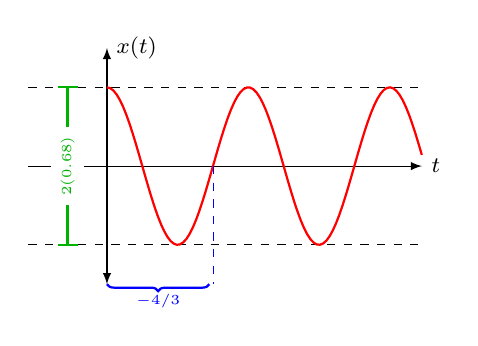
\begin{tikzpicture}[>=latex]
	\draw [<->] (0,-1.5) -- (0,1.5) node [right] {\footnotesize \(x(t)\)};
	\draw [->] (-1,0) -- (4,0) node [right] {\footnotesize \(t\)};
	\draw [dashed] (-1,1) -- (4,1);
	\draw [dashed] (-1,-1) -- (4,-1);
	\draw [thick , red , domain=0:4, samples = 100] plot(\x , {cos(3.5*\x r)});
	\draw [green!70!black,|-|, thick] (-0.5,-1.02) to node[midway,rotate=90, fill=white] {\tiny \(2(0.68)\)} (-0.5,1.02);
	\draw [snake = brace, mirror snake, thick , blue] (0,-1.5) to node[below,midway] {\tiny \(-4/3\)} (1.3,-1.5);
	\draw [dashed, blue] (1.35,0) --++ (0,-1.5);
\end{tikzpicture}

\end{document}
